% Activate the following line by filling in the right side. If for example the name of the root file is Main.tex, write
% "...root = Main.tex" if the chapter file is in the same directory, and "...root = ../Main.tex" if the chapter is in a subdirectory.
 
%!TEX root =  

\chapter{Project Evaluation}\label{eval}

\minitoc


The final phase of the project consists of evaluating the actual outcome of
the project work and the processes that have led to the outcome. It
seeks to answer questions such as:

\begin{itemize}
\item Has the project acheived its major objectives?
\item In what areas could a better result have been achieved?
\item What could be done differently to acheive a better result?
\item How well did planned resource use reflect actual resource use?
\end{itemize}

The first section evaluates the software system in terms of the
objectives and requirements worked out prior to design and
implementation.  Sections \ref{toolseval} and \ref{resourceUse}
evaluate the appropriateness of the tools used in developing the
system and the resources committed to the project in manhours relating
to the original project plan. Finally, section \ref{courseEval}
evaluates the course as a whole.

\section{Software Evaluation}

This section contains the project team's evaluation of the software
system that has been produced.

\subsection{Key Objectives}

As discussed in Section~\ref{mandateObjectives}, the main objectives of the project were:

\begin{enumerate}
\item\label{itemTestFW} Implementing a testing framework of CBR based privacy agent that is able to make privacy decisions based on previous user behavior.
\item\label{itemCollaborative} Implement the community system/collaborative filtering part of the agent.
\item\label{itemExtend} Extend the system to other standards for machine readable privacy policies.
\item\label{itemBrowser}Implement the system as a browser plugin. 
\end{enumerate}

Objective~\ref{itemTestFW} was considered the clearly most important for the project, being a prerequisite for the remaining objectives. The fuctional requirements section (Section~\ref{funcRequirements}) in requirements specification goes further in detail on what the first objective entails.

\subsection{Evaluation}
The project team realized quickly that there were insufficent resources to meet Objectives 3-4, so focus was shifted to the first objective while, there was planned for working towards the second objective at the end of the project period. With respect to the first objective, the \emph{current Privacy Advisor system provides all the features listed in the requirements specification}. The second objective is partially realized. The core Privacy Advisor system has functionality extending the CBR for networking, and work on a collaborative filtering system has been started on a server machine at NTNU. The features supported by this system is however limited.


%%TODO: refer to testing results

\section{Tools}\label{toolseval}

Referring to choices discussed in section~\ref{DevTools}, the key
software tools and languages used are Java, Git, and Google
Docs. 

\subsection{Programming and Implementation}

\subsubsection{Java}
The choice of programming language for the project was very much up to the
project team as the customer had no particular preference, and the
project did not require anything beyond what is catered for by most
general purpose languages. \textbf{Java} was therefore selected 
selected as implementation language based on the following points:

\begin{itemize}
\item All team members had some previous experience in Java
  programming from previous coursework.
\item Good documentation and a large amount of third party libraries
  available on the web.
\end{itemize}

While all team members did have a Java programming background, there
were clearly vast differences in skill levels. This was the cause of
some frustration and extra work. In retrospect, more time should have been spent
on clarifying background and interests of each team member so as to
better allocate workload. Some will also argue that a more
"light-weight" programming language, such as Python, would have been a
better choice, even despite the lack of previous experience.

\subsubsection{Git/GitHub}
Git was chosen as version control system (VCS) using GitHub as 
the repository for source code hosting. Several team members had only marginal experience with
VCSs and did not commit to learning this in a serious manner, which
led to somewhat slow progress in the start. However, once these problems
were resolved, it can be agreed that Git has served its purpose well.


\subsection{Reporting and Organizational Tools}
Google Docs was used as repository for all "temporary" documents such
as agendas, status reports, drafts and so forth. All "major"
documents were typeset in \LaTeX and stored at the GitHub repository.

\subsubsection{Google Docs}
There were no significant issues with Google Docs. It provided a good
framework for sharing binary files such as spreadsheets, presentations and so forth which
are not catered well for by most version control systems.


\subsubsection{\LaTeX}
Being the de-facto typesetting system for academic writing, and the
only one that some group members had experience with, \LaTeX was
chosen for writing the final report as well as all phase documents. As
with GitHub, though to a lesser extent,  there was a lack of commitment to learning by certain
group members, causing frustration and extra work on a later stage
in the project.


\section{Resource Use}\label{resourceUse}

 Figures~\ref{actualPlannedCuml} and \ref{perActivity} illustrate
the discrepancies between actual and planned time use on all
activities, both cumulative over time and over each phase of the
project. It is updated as by the end of the last week of the project.

\begin{centering}
  \begin{figure}[h!]
    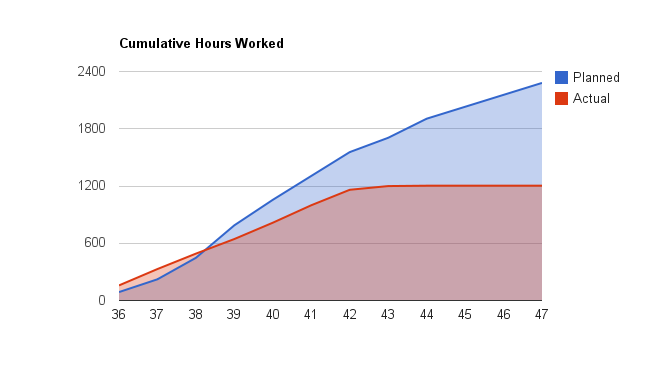
\includegraphics[width = \textwidth]{Evaluation/actual_v_planned_cuml}
    \caption{Actual vs. planned time. Cumulative over project span.}
    \label{actualPlannedCuml}
  \end{figure}
\end{centering}

As shown in Figures~\ref{actualPlannedCuml} and \ref{perActivity}, there
are a few important discrepancies between the project plan and how the
project indeed turned out. Firstly, there was a shortage of
approximately 300 hours. This was quite evenly spread among most team
members, with the exception of the team members with administrative
responsibilities who had a significantly higher workload. The uneven
workload also reflects an uneven background in academic writing which
meant a large portion of the workload with this report was taken on by
a few select team members. It could also be argued that there simply
too many group members assigned to the project for everyone to be able
to properly contribute, in the sense that for each project phase there
was only a limited amount of work, and having too many group members
working on the same tasks would simply generate too much overhead.

Secondly, while the percentage workload between activities was quite
well anticipated, there were some noticeable exceptions. One key
pattern to notice is that while the design and implementation related
activities required less time than initially planned, administrative
work and planning required more work than planned. The overrun is most
obvious for the administrative tasks part. One important lesson to
take away from this is that a project team of a given size does need a
major amount of administrative work. Another important reason for this
overrun was initial problems with setting up the code repositories. 

\begin{centering}
  \begin{figure}[h!]
    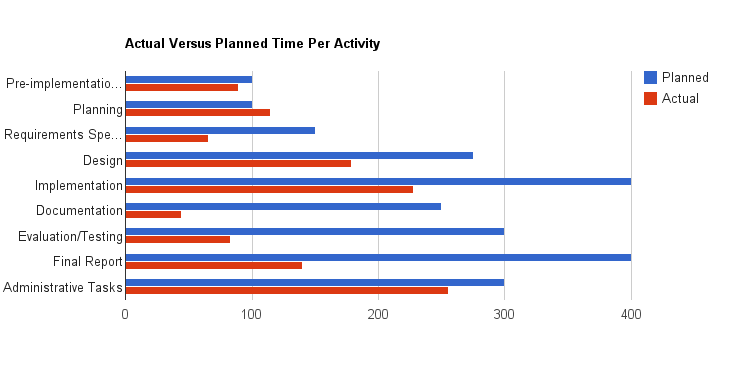
\includegraphics[width=\textwidth]{Evaluation/time_per_activity}
    \caption{Actual vs. planned time. By project phase, in hours.}
    \label{perActivity}
  \end{figure}
\end{centering}

With respect to the relatively fewer hours spent on designing and
implementing the system, a portion of this can be explained by the
fact that a major portion of the design was clear from the beginning
given that the system was to be based on the CBR framework. This and
the fact that Java was decided on early on as programming language,
severely limited the possible designs available. The implementation
phase also required fewer hours than expected. This was in part due to
the fact that the team did not realize all the objectives that were
set (networking is only partially completed), and that work was divided
well among team members. Interfaces were also built quite early on in
the project so that adding on modules to existing code proved simple. 


\begin{centering}
  \begin{figure}[h!]
    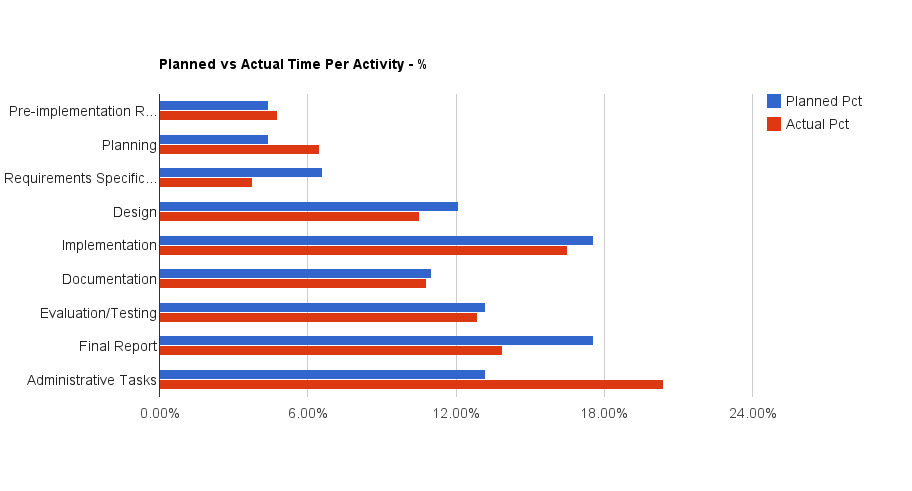
\includegraphics[width=\textwidth]{Evaluation/time_per_activity_pct}
    \caption{Actual vs. planned time. By project phase, in percentage of total time.}
    \label{perActivityCUml}
  \end{figure}
\end{centering}

\section{Risks that Occurred}\label{courseEval}

Referring to the discussion in section~\ref{riskReport}, it can be said
in retrospect that few of the anticipated risks occurred, at least
with major consequences. Some problems occurred building a P3P
parser (risk item 3), causing some initial delays as it took longer time than
anticipated to get the system fully working. This problem was in part
due to some unclear notions in the specification of the dataobjects
storing P3P objects.

Furthermore, the project has not proceded without any conflicts. While
roles and responsibilities were agreed on early on in the project
phase, it turned out that these initial assignments did not distribute the
workload very evenly. 
